\chapter{Introducción}

\section{Conceptualización}

La escuela (salesiana) al alcance de los más necesitados en Irapuato es un bachillerato tecnológico que se pretende crear en dicha ciudad con el doble objetivo de brindar una capacitación técnico-académica de calidad a nivel bachillerato y de ofrecer una educación integral en valores según el sistema educativo de Don Bosco a los jóvenes más necesitados.

\subsection{Origen de la Idea}

La idea original nace en el seno de la Comunidad Salesiana <<María Reina de Irapuato>> la cual ante la problemática social enfrentada por las familias en esta ciudad, tales como  la ruptura familiar, las adicciones y el analfabetismo, propone la realización de este proyecto, al validar que, ante la interrogante <<¿Qué estamos haciendo por los pobres?>>, no se tiene una respuesta plenamente satisfactoria puesto que las estadísticas locales, la entidad presenta elevados índices en las variables antes mencionadas.\citep{Morales09}

Ante esta situación, el Pbro. Edmundo Morales Romero, S.D.B, sacerdote salesiano miembro de dicha comunidad, destaca la existencia de numerosas razones por las cuales es urgente emprender una labor educativa a fondo y de largo alcance que impacte en el desarrollo local dentro de su ámbito de influencia en primera instancia y en un futuro próximo sea susceptible de reproducción en las demás entidades del país.

Este modelo pretende cubrir desde un sector cuyo nivel económico le permita pagar una colegiatura hasta aquel para el que es del todo imposible hacerlo por si mismo.

Al bachillerato podrán ingresar todos aquellos que hayan acreditado la secundaria. Las clases las tomarán todos juntos evitando todo tipo de discriminación y eliminando una barrera de la historia reciente en nuestro país: la diferencia entre los que van a escuela de paga y a escuela pública.

El perfil de egreso es el de bachillerato de alta calidad con una carrera técnica adecuada a las características de la región.

\subsection{Notas Distintivas}
\label{sub:intro:NotasDistintivas}

La escuela tiene como rasgos distintivos aquellas características del modelo educativo de Don Bosco, y que pueden resumirse en 5:

\begin{description}
	\item[Sistema preventivo] En contraposición al sistema represivo, se trata de ganar a los estudiantes con amabilidad para orientarlos al bien. A los 9 años, Don Bosco tuvo un sueño en el que Jesús le decía: \emph{no con golpes, sino con la mansedumbre y la caridad deberás ganarte a estos tus amigos}\footnote{San Juan Bosco, Memorias del Oratorio en \citep{Canals95}}.

	\item[Acompañamiento] Los jóvenes nunca están solos, incluso en los ratos de descanso y esparcimiento siempre hay alguien que los acompaña y convive con ellos.
	
	\item[Formación en valores] El sistema preventivo, en palabras de Don Bosco, sólo funciona si se basa en el Evangelio, en una sólida vida interior apoyada en los sacramentos. De aquí se desprende todo lo demás\footnote{San Juan Bosco, en \emph{El Sistema Preventivo en la Educación de la Juventud} (1877) nota 1, \citep{Canals95}. El texto de la nota puede verse íntegro en el Apéndice \ref{ap:preventivo}, página \pageref{ap:preventivo}}.

	\item[Quitar barreras de discriminación] En un mismo salón de clase convivirán jóvenes de todos los estratos sociales, a los cuales se les brindará el mismo trato promoviendo la amistad entre ellos.

	\item[Formación para el trabajo] Mediante las carreras técnicas y los talleres se procurará que los jóvenes tengan la posibilidad de conseguir un empleo ya sea de tiempo parcial para seguir estudiando o si las circunstancias se imponen, de tiempo completo.
\end{description}

\section{Objetivos}

\subsection{Objetivo General}
\label{sub:ObjetivoGeneral}

El objetivo general del presente trabajo es verificar la viabilidad financiera de la Escuela Salesiana.
% así como identificar las fuentes de financiamiento que requiere para operar.

%Siendo un proyecto que persigue un fin social antes que lucrativo, se distinguen dos tipos de viabilidad: la financiera y la social.

La viabilidad financiera se entiende en el sentido de que el bachillerato puede
%simultáneamente cumplir su función social y
ser un negocio redituable.

%Sin embargo, la viabilidad más importante que se desea alcanzar es la social, en la cual el proyecto se vuelva autónomo para operar, es decir, que los ingresos superen o al menos equiparen a los costos una vez cubiertas las obligaciones de deuda que se adquieran a la par que proporciona un beneficio a la comunidad local.

\subsection{Objetivos Específicos}

\begin{itemize}
	\item Determinar la estructura de costos
	\item Determinar las fuentes de ingresos
	\item Identificar el punto de equilibrio
	\item Verificar la viabilidad financiera y social del proyecto
	\item Establecer un principio ordenador para el resto de los planes a elaborar para poner en marcha el proyecto.
\end{itemize}

\section{Alcances y Limitaciones}

\subsection{Alcances}

Para hacer realidad este proyecto, se está integrando un plan a nivel macro, que a su vez contenga siete sub proyectos o planes, los cuales son: plan financiero, plan pedagógico, plan de capital humano, plan de relaciones públicas, plan organizacional, plan de infraestructura y plan de puesta en marcha.

El presente trabajo abarca únicamente el plan financiero y los aspectos que directa o indirectamente impactan en él.

Quedan fuera del alcance de este proyecto los siguientes planes: pedagógico, capital humano, relaciones públicas, organizacional, infraestructura y puesta en marcha.

\subsection{Limitaciones}

El modelo de financiamiento es múltiple: aportaciones directas (colegiaturas), fondos privados, apoyos públicos, servicios a empresas, entre otros.

Se cobrará una aportación monetaria en función de las capacidades de cada alumno. El objetivo es financiar a los jóvenes de escasos recursos mediante las aportaciones de los estudiantes con posibilidades económicas.
Se buscarán fondos privados para becas e infraestructura en diversas modalidades: apadrinar alumnos con buenas calificaciones, apoyos para proyectos específicos: laboratorios, talleres, etc.; apoyos en especie.

Se intentará obtener apoyos públicos en función de la labor social que se realiza a través de programas como Oportunidades, Practica-Trabaja, Lazos, Bécalos, Prepa Sí, etc.

Entre otras actividades para obtener ingresos se contemplan: prácticas profesionales patrocinadas por empresas (venta de servicios de acuerdo a carrera técnica y necesidades de las empresas locales); programas de reciclaje; rifas, noches coloniales y eventos de sano entretenimiento, etc.

Como actividades formativas y simultáneamente ahorradoras se consideran las siguientes: aportaciones en especie de los miembros de la comunidad, jornadas de limpieza, pintura y reparación; servicio en la cooperativa (tienda de la escuela), etc.

\section{Prefactibilidad}

\subsection{Aspectos Previos - Situación Actual}
\label{sub:Intro:AspectosPrevios}

El estado de Guanajuato enfrenta diversos problemas sociales derivados de una oferta educativa insuficiente
(Cf. \citep{Morales09}):

\begin{description}
	\item[Educación] Guanajuato es una de las entidades con mayor índice de analfabetismo a nivel nacional. Concentrándose la mayor cantidad de analfabetas \emph{en las zonas urbanas}.\footnote{Seg\'{u}n el Conteo de Poblaci\'{o}n y Vivienda 2005 \citep{Inegi2005}, Guanajuato ocupa el quinto \emph{\'{u}ltimo} lugar en escolaridad con 7.1 a\~nos en promedio contra 8.1 nacional.}
	\item[Desempleo] El desempleo asciende al 37\% de la población económicamente activa.
	\item[Niños de la calle] Guanajuato es de los principales estados receptores de niños de la calle.
	\item[Ruptura familiar] Guanajuato está en el 4º lugar de divorcios, ha aumentado un 400\% en estos últimos años, con el consiguiente semi abandono de los niños.
	\item[Delincuencia] Al igual que el resto del país, la entidad padece un incremento en los índices delictivos y de violencia.
\end{description}

\subsection{En Caso de no Llevarse a Cabo}

En caso de no llevarse a cabo el proyecto, estos índices aumentarían con grave daño a la sociedad local.

Por otra parte, el gran desarrollo industrial del Estado se vería afectado y la comunidad no podría aprovechar este beneficio, al no contar con la preparación técnica necesaria, las empresas contratarían personal foráneo para cubir sus necesidade de talento humano.

\subsection{Ubicación}

Se cuenta con un inmueble ubicado en la zona centro de Irapuato, abarca toda la manzana delimitada por las calles: Díaz Ordaz, Francisco Sarabia, Río Grijalba y Lázaro Cárdenas, se puede observar una foto satelital en la figura \ref{fig:ubicacion}.

\begin{figure}
	\centering
	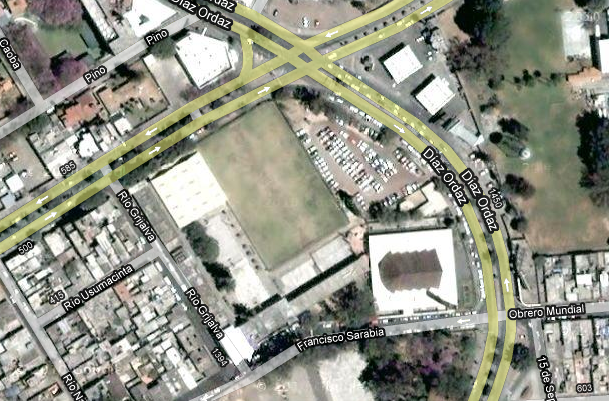
\includegraphics[scale=0.5]{images/localizacion}
	\caption[Fotografía satelital y ubicación del inmueble.]{Fotografía satelital y ubicación del inmueble.\newline Fuente: \citep{GoogleMaps2010}}
	\label{fig:ubicacion}
\end{figure}

\subsection{Evaluación Financiera Previa}

\subsubsection{Infraestructura Actual}

Se cuenta con un inmueble adaptado como escuela, al cual, actualmente no se le da este uso; aunque requerirá modificaciones menores ya tiene la capacidad de atender a más de 1,000 alumnos en 40 aulas.

La superficie del inmueble es de 14,452 $m^2$ con un valor aproximado de \$ 3.4 millones de pesos; los edificios están valuados en \$ 2.4 millones de pesos aproximadamente.

%\footnote{Valor estimado con base en el precio por metro cuadrado promedio en Irapuato \citep{AM2010}}.

\subsubsection{Beneficio Social}
\label{sub:sub:Beneficio:Social}

La intención es cubrir al menos un 40\% del alumnado con alguna beca. Por comparación, un bachillerato salesiano en Jalisco orientado como \emph{escuela privada} otorga un 20\% en becas.

Considerando la capacidad actual del inmueble el beneficio social que se espera obtener es el equivalente a 400 jóvenes atendidos de forma completamente gratuita. Sin embargo, la intención es distribuir las becas utilizando porcentajes, por lo que la cobertura real deseada es que más de la mitad de la población estudiantil se vea beneficiada con algún tipo de beca.

Por otra parte, la educación en valores basada en el sistema preventivo de Don Bosco beneficiará todos los estudiantes y a sus familias.

\subsubsection{Capacidad actual}

Se pretende dividir a los alumnos en grupos de 30 estudiantes como máximo. De acuerdo con el sistema salesiano, esto da como resultado un total de 37 personas atendiendo directamente a los estudiantes.

La colegiatura estándar en la región es de \$3000.00 mensuales, lo cual, aplicado a 600 estudiantes durante un año da como resultado un monto de \$21,600,000.00. A esta cantidad habrá que añadir lo que se obtenga mediante donativos y patrocinios.

\subsubsection{Patrocinios}
\label{sub:Patrocinios}

Las experiencias similares en Saltillo y San Luis Potosí\footnote{Entrevista con el Pbro. Edmundo Morales Romero, S.D.B., 11 de septiembre de 2011} muestran que esta clase de proyectos son bien recibidos por los industriales locales; en efecto, en ambas entidades, los grupos industriales realizaron aportaciones en efectivo y en especie a tal grado que incluso donaron los terrenos a cambio de adaptar los planes de estudio a sus necesidades.

Irapuato se ubica en el centro del eje industrial de Guanajuato, el cual incorpora a las ciudades de León, Silao, Irapuato y Salamanca. En toda esta zona existen diversos parques industriales e industrias de todo tipo. Próximamente se abrirá una planta de fabricación de componentes espaciales, la cual estará necesitada de mano de obra calificada. Todas estas industrias son candidatos a ser patrocinadores del proyecto por así convenir a sus intereses.
